\documentclass[glossarios,figuras,sumario]{setup/obnzip2}

\usepackage[math,bold,env]{curtatex}
\usepackage{siunitx}
\usepackage{titlesec}
\usepackage{float}
\usetikzlibrary{positioning,trees,mindmap}

\DeclareDocumentCommand{\quote}{m}{%
	``#1''%
}
\DeclareDocumentCommand{\citeay}{s m}{{\IfBooleanT{#1}{\bfseries}\citeauthor{#2} - \citeyear{#2}}}
\NewDocumentCommand{\citem}{s m}{\item[{\def\seleccite{\bfseries}\cite{#2}}]}
\NewDocumentCommand{\papersec}{m}{%
	\stepcounter{subsubsection} \noindent\textit{\vspace*{1ex}\\\Alph{subsubsection}.\hspace*{0pt-\widthof{\Alph{subsubsection}}} \hspace{1em} #1} \vspace*{1ex}
}
\let\citet\textcite

\definecolor{tomographycolor}{RGB}{0, 0, 0}
\definecolor{ssfinvcolor}{RGB}{0, 0, 0}

\def\seleccite{\relax}
\makeatletter
	\NewDocumentCommand{\ProcessKeyColor}{>{\SplitList{,}} m}{%
		\ProcessList{#1}{\@MatchKeyColor}%
	}
	\NewDocumentCommand{\@MatchKeyColor}{m}{%
		\ifkeyword{#1}{\hypersetup{citecolor=#1color}}{}%
		\ifkeyword{selec}{\seleccite}{}%
	}
\makeatother

\AtEveryCitekey{\ProcessKeyColor{tomography,ssfinv}}
	
\def\tline{\hline\vphantom{\rule{0.4pt}{1.2em}}}
\def\ttline{\hline\vphantom{\rule{0.4pt}{1.2em}}}

\pdfsuppresswarningpagegroup=1
\BiblatexSplitbibDefernumbersWarningOff




\begin{document}	
	\section{Campo de Velocidade do Som}
\label{sec:campo_de_velocidade_do_som}

Embora seja comum considerar a velocidade do som na água como uma constante, em torno de $1500 \si{\meter/\second}$, essa aproximação é inválida para ambientes de grande escala \cite{kieffer_sound_1977,trusler_determination_2017,li_sound_2015,pinson_sound_2010}. Muitas propriedades podem afetar a velocidade do som na água, como temperatura, pressão estática, e salinidade, além de correntes marítimas \cite{wilson_speed_1959,medwin_fundamentals_1999,mcdougall_getting_2011,delgrosso_new_1974}. À medida que essas propriedades variam na massa de água, a velocidade também varia, criando um \gls{ssf} na massa de água. Embora o termo \gls{ssp} \cite{li_acoustic_2019,li_sound_2015,pinson_sound_2010} também seja comumente usado, ele geralmente se refere ao cenário de estimativa 1D.

%\subsection{Propagação sonora na água}
\subsection{Princípios}

O conhecimento da velocidade do som em cada ponto de uma massa de água permite o conhecimento das propriedades --- como caminho, fase, amplitude, e tempo de trânsito --- de uma onda que se propaga por esse meio.

\subsubsection*{Relação do SSF com parâmetros TPS}

Como já citado, as propriedades de \gls{tps} afetam a velocidade do som na água, atuando de maneiras diferentes. Essa relação é conhecida, e trabalhos iniciais que tratavam da reconstrução do \gls{ssf} visavam estimar essas propriedades principais, bem como a relação entre elas e a velocidade do som. Trabalhos como \cite{wilson_speed_1959,medwin_fundamentals_1999,mcdougall_getting_2011,delgrosso_new_1974,chen_speed_1977,wong_speed_1995,roquet_accurate_2015,mackenzie_nineterm_1981,wilson_equation_1960} operaram dentro dessa estrutura, alguns ainda sendo usados atualmente para modelar o comportamento de correntes marítimas em escala global.

Modelos como os desenvolvidos por \cite{wilson_equation_1960,mackenzie_nineterm_1981,delgrosso_new_1974} relacionam diretamente as variáveis de \gls{tps} com a velocidade do som por meio de funções polinomiais, tendo sido obtidas empiricamente com base em expedições de medição dos parâmetros \gls{tps}, e da velocidade do som. Estes modelos são considerações formulações fechadas, pois a \gls{ssf} pode ser calculada usando um número finito de operações padrão.

O modelo TEOS-10 \cite{mcdougall_getting_2011} é outro método para estimação do \gls{ssf}, resolvendo equações químico-termodinâmicas para determinar a distribuição de velocidade adequada, em função da energia. Na modelagem são resolvidas uma série de equações interconectadas que envolvem a composição química detalhada da água e o equilíbrio térmico. Também baseia-se em parâmetros de \gls{tps} modificados (temperatura conservativa, pressão hidrostática e salinidade absoluta), mas não é uma formulação fechada (como nos modelos desenvolvidos por \cite{wilson_equation_1960,mackenzie_nineterm_1981,delgrosso_new_1974}).

\subsubsection*{Refração}

Um efeito importante, quando tratando de ondas sonoras que atravessam um ambiente com velocidade sonora variável, é o efeito da refração, em que o caminho que a onda percorre não é necessariamente retilíneo. Por estarmos trabalhando com corpos d'água de grandes dimensões (podendo chegar à casa de quilômetros de largura e/ou profundidade), a velocidade do som também pode variar muito e de forma imprevisível ao longo do corpo d'água, necessitando que a refração seja considerada.

Esse efeito está fortemente ligado ao princípio de Fermat de tempo mínimo \cite{se-yuen_closer_1986}, que dita que uma onda (modelada por um raio) que atravessa um meio sempre buscará o menor tempo de viagem. Isso faz com que conhecer o SSF torna o tempo de primeira chegada da onda previsível. Se assumirmos que o \gls{ssf} varie discretamente de velocidade (uma aproximação que será explorada adiante), o princípio de Fermat pode ser representado pela lei de Snell \cite{perrine_fermats_1961}, descrevendo a mudança de ângulo (refração) da onda ao atingir uma interface (discreta) entre dois meios com velocidade do som diferentes.

Por outro lado, a refração pode ser tratada pelo princípio de Huygens, \cite{bormann_seismic_2012}, que modela cada ponto em uma frente de onda como uma fonte sonora secundária. A interação entre essas fontes sonoras virtuais produz o envelope da onda ao longo do tempo e, com isso, gera os mesmos efeitos de refração.

\subsection{Estimação do SSF por inversão}
\label{subsec:sec1:estimacao_ssf_por_inversao}

Como discutido, é possível modelar o \gls{ssf} a partir dos parâmetros de \gls{tps}. Contudo, a estimação desses parâmetros é muitas vezes inviável na prática. Dessa forma, a maioria das abordagens modernas para a reconstrução do \gls{ssf} evita estimar essas propriedades e trata a estimação como um problema de inversão. Parte-se do princípio de que, como o conhecimento do \gls{ssf} permite calcular a trajetória e as propriedades de uma onda que atravessa o meio; então o conhecimento dos caminhos (e/ou das propriedades) permite estimar o \gls{ssf}.

A maioria das técnicas utiliza fontes e receptores sonoros dentro do corpo d'água e, comparando as propriedades das ondas produzidas e recebidas, estima o caminho das ondas; e, a partir disso, obtém uma reconstrução para o \gls{ssf}. Diferentes técnicas tratam esse problema de inversão usando uma vasta gama de tipos de dados e medições, bem como abordagens matemáticas e modelagens distintas.

\subsubsection*{Tomografia de Tempo de Trânsito}

A \gls{ttt} \cite{bormann_seismic_2012,stefanov_travel_2019} é um dos métodos de inversão mais simples para estimativa do \gls{ssf}. Ela utiliza a diferença no tempo de chegada dos sinais acústicos nos sensores, exigindo uma distribuição espacial de fontes e receptores para resolução espacial suficiente.

Ela se baseia em uma discretização espacial do \gls{ssf} em células (ou às vezes camadas), em que a velocidade do som é considerada constante dentro de cada célula; e no princípio de Fermat de tempo mínimo, relacionando o \gls{ssf} ao tempo de primeira chegada da frente de onda em cada ponto do espaço.

No processo iterativo que rege a \gls{ttt}, calcula-se o comprimento dos percurso das ondas em cada célula, resultando em um sistema de equações usado para estimar/iterar o \gls{ssf}. Adaptações do \gls{ttt} incluem a hipótese de o \gls{ssf} se comportar aproximadamente como conhecido, isso sendo inserido como uma regularização, parametrização, ou permitindo uma decomposição modal.

Suas principais vantagens são robustez, simplicidade, e eficiência computacional, a último permitindo implementação em tempo real. No entanto, a \gls{ttt} depende de um posicionamento e sincronização exata dos dispositivos (fontes e receptores), e sua suposição de discretização resulta em resolução limitada.

\subsubsection*{\ingles{Matched Field Inversion}}

Na técnica \gls{mfi} \cite{dosso_bayesian_2011}, é utilizada (primariamente) a informação de pressão sonora medida nos receptores. Essa informação é comparada com modelos de pressão acústica para diferentes \gls[SSFs]{ssfs}, e esses \gls[SSFs]{ssf} são adaptados e iterados de forma a minimizar o erro entre os dados de pressão sonora obtidos e a pressão sonora estimada.

Essas técnicas são semelhantes à formação de feixe (\textsl{beamforming}), utilizada em diversas áreas como acústica e processamento de sinais \cite{schmidt_environmentally_1990,brienzo_broadband_1993}, sendo que ambas --- \gls{mfi} e \textsl{beamforming} --- exploram a correlação espacial entre os receptores e suas medições, modelando o campo acústico dessa modelagem espacial.

O \gls{mfi} também emprega a decomposição modal dos sinais, com cada modo se comportando de maneira diferente na água. Dessa forma, ela incorpora informações mais complexas sobre os sinais, como amplitude e fase, dependendo não apenas do tempo de trânsito. Entre suas vantagens destacam-se o melhor aproveitamento dos dados obtidos, a resolução espacial aprimorada (em comparação com o \gls{ttt}) e a maior robustez ao ruído devido ao processamento coerente dos sinais obtidos nos receptores. No entanto, ela requer informações espaço-temporais sobre a fonte e os receptores, como diretividade e comportamento da potência em função da frequência. Além disso, não é adequada para corpos d'água muito grandes, visto que um corpo maior resultaria em um modelo de pressão sonora com uma quantidade exponencialmente maior de parâmetros. Essa técnica também é computacionalmente muito custosa.

\subsubsection*{\ingles{Full-Waveform Inversion}}

As técnicas de \gls{fwi} \cite{virieux_overview_2009,fichtner_multiscale_2013} visam a reconstrução da forma de onda dos sinais presentes no \gls{ssf}, considerando diversos comportamentos que são negligenciados pelas técnicas mencionadas anteriormente. Nesse método, o erro entre as formas de onda estimadas e medidas é minimizado iterativamente, buscando o \gls{ssf} que melhor represente os dados obtidos. Essa técnica pode operar no domínio do tempo, ou no da frequência.

Dado isso, a técnica \gls{fwi} está entre as que melhor utilizam os dados disponíveis nos receptores, resultando no \gls{ssf} mais fiel, além de aproveitar ao máximo os sinais disponíveis. Entretanto, devido à consideração de interações complexas entre os sinais e múltiplos caminhos de onda, há um aumento significativo na complexidade matemática e computacional. Isso, aliado à não linearidade do problema, resulta em uma técnica muito complexa e por vezes inviável, que também requer uma estimativa inicial adequada dos parâmetros para sua robustez e convergência.

\subsection{Limitações do projeto relevantes à estimação do SSF}

Dentro do presente projeto do OBNZip 2, surgiram algumas restrições quanto aos dispositivos (fontes e receptores) que serão utilizados, e tipo de informação que pode ser obtida.

\begin{enumerate}[itemsep=0pt]
	\item Transceptores são alocadas ao longo do leito oceânico.
	\item Transceptores são alocados próximo à superfície, em profundidades não superiores a $500\si{\meter}$ em situações de água profunda.
	\item Fontes se comunicam acusticamente com receptores, e o tempo de trânsito dessa comunicação é medido.
	\item Apenas a informação de tempo de trânsito é obtida na comunicação (considerando os dispositivos atualmente alocados).
\end{enumerate}

Embora os dispositivos alocados no leito e na superfície são ambos transceptores (isto é, ambos emitem e recebem comunicação), será convencionado que os dispositivos no leito oceânico serão \gls{fontes}, e os na superfície serão \gls{receptores}. Isso simplifica o modelo matemático e a descrição do problema, e deve ser considerado futuramente ao utilizar os desenvolvimentos apresentados.

\subsubsection*{Fontes sonoras}

É desejado utilizar os \gls[OBNs][nós de leito oceânico][Ocean Bottom Nodes]{obn} (inclusive especificamente \ingles{On Demmand} \gls[OBNs]{obn} da Sonardyne) que já estão dispostos no leito oceânico como as fontes sonoras, de forma a não necessitar a construção e implantação de novos equipamentos.% Isso leva a outras restrições, como quanto às frequências sonoras que podem ser utilizadas (limitadas às produzidas pelos OBNs).

\subsubsection*{Receptores}

Os receptores serão implementados por meio de expedições com \ingles{streamers}, \gls[ROVs][veículos operados remotamente][Remotely Operated Vehicles]{rov} ou outros dispositivos, em que esses se comunicam com os \gls[OBNs]{obn}. Embora o problema seja matematicamente modelado como utilizando diversos receptores, na prática isso é implementado como um único (ou alguns poucos) receptor(es), com esse sendo alocado em posições diferentes.

Uma restrição relacionada aos receptores é quanto ao seu posicionamento: dado que o custo de uma expedição está atrelado à profundidade que os receptores serão utilizados (mais caro levá-los até áreas mais profundas, além de uma complexidade maior), deseja-se limitar a profundidade na qual eles podem ser utilizados. Em específico, é de interesse que os receptores estejam limitados a profundidades de $500\si{\meter}$, como alinhado com a Petrobras.

\subsubsection*{Comunicação e tempo de trânsito}

Como o interesse inicial é a utilização da comunicação acústica entre os dispositivos (ao menos nesse primeiro momento), a informação disponível que pode ser utilizada é restrita ao tempo de trânsito entre fontes e receptores.

Tecnicamente, o esquema que será utilizado envolve dispositivos transceptores, operando simultaneamente como fonte e receptor: o dispositivo A emite o sinal; o disp. B recebe, processa, e responde; e o disp. A recebe essa resposta, medindo o tempo de viagem A--B--A. Contudo, por questões de simplificação da modelagem, assume-se que o tempo de viagem A--B é igual ao tempo de viagem B--A, bem como que o disp. B é a fonte, e o disp. A é o receptor.

Também é assumido que não ocorra comunicação entre fonte-fonte (não se sabe o tempo de trânsito entre OBNs), nem entre receptor-receptor; apenas fontes e receptores.

\subsection{Diferenças entre os casos 1D e multi-dimensionais} % Adicionado por sugestão do Luis

Anteriormente, foram apresentados os casos 1D e multi-dimensionais, sem que esses forem profundamente tratados, em particular quanto às suas peculiaridades. Trivialmente, a passagem do caso 1D para o 2D (e do 2D para o 3D, e desse para o 4D) leva a um aumento na complexidade do problema, atrelado tanto ao aumento do número de unidades a serem estimadas no ambiente; mas também um aumento na complexidade das interações entre as ondas que trafegam o ambiente e as células que o compõem, com essas podendo viajar em mais direções, e podendo tomar caminhos diferentes.

Além disso, a alocação de dispositivos está intimamente ligada à estrutura que pode ser estimada. Por exemplo, em um caso com dispositivos alocados em uma única coluna e alinhados verticalmente, não haverá medições do ambiente além dessa coluna (em particular de informações de tempo de primeira chegada), impossibilitando qualquer tipo de estimação que não seja uni-dimensional. Portanto, de maneira geral, a dimensionalidade da estimação está limitada à dimensionalidade da alocação dos dispositivos.

\subsection{\textsl{Mindmap}}

A figura da \cref{fig:mindmap_sec1} mostra um \textsl{mindmap} dos conceitos expostos ao longo da \cref{sec:campo_de_velocidade_do_som}, de forma a dispor graficamente a organização das informações apresentadas. A cor de cada nó indica o conceito-pai dele.

\begin{figure}[!t]
	\centering
	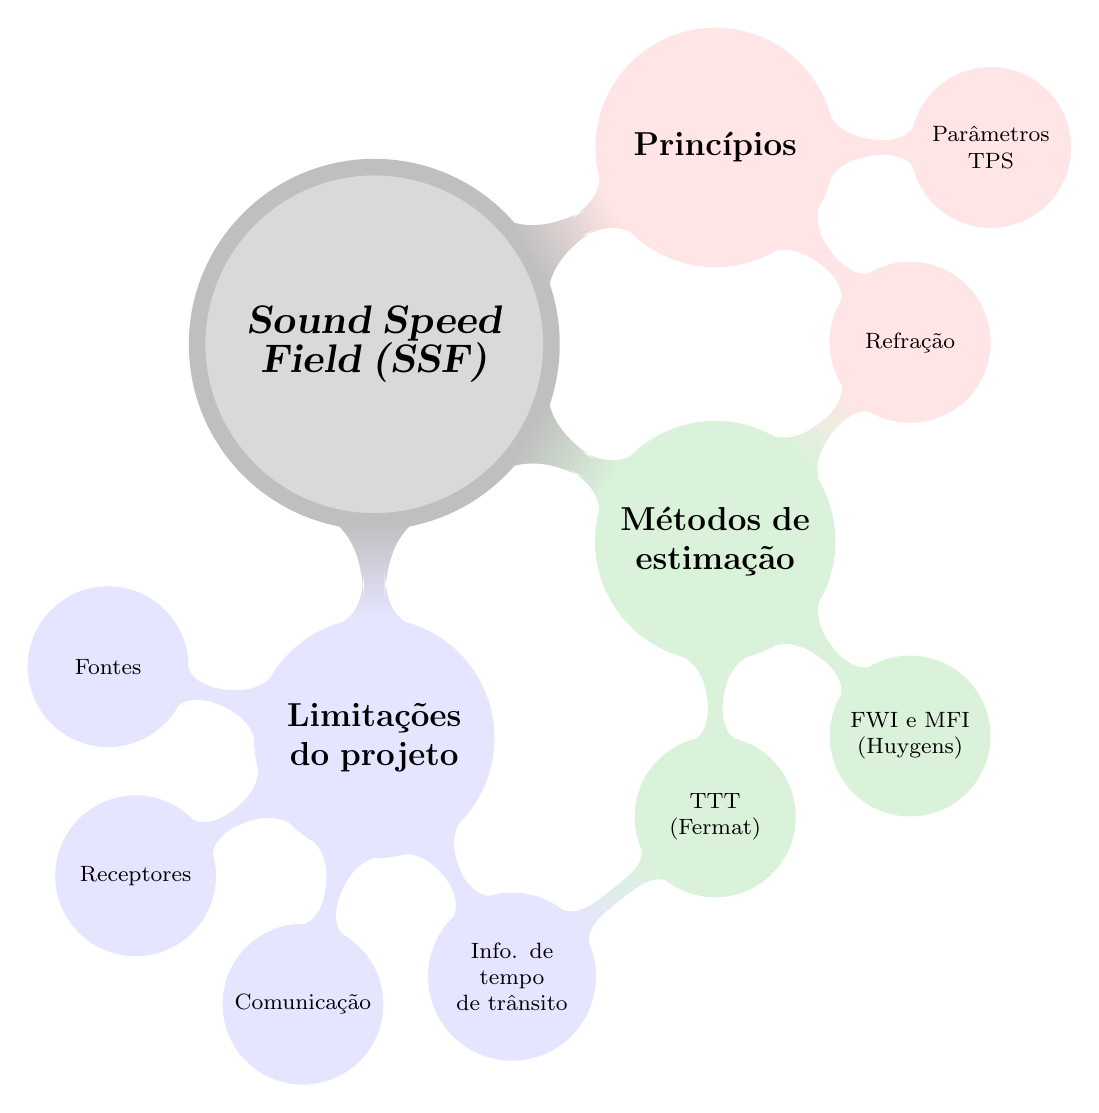
\begin{tikzpicture}[
		mindmap,
		text width=2.5cm,
		align=center,
		every node/.style={concept},
		concept color=gray!50,
		level 1/.append style={
			level distance=5cm,
			minimum size=3cm,
			text width=2.8cm,
			font=\large,
		},
		level 2/.append style={
			level distance=3.5cm,
			minimum size=2cm,
			text width=1.8cm,
            font=\footnotesize
		},
		level 3/.append style={
			level distance=3.5cm,
			minimum size=2cm,
			text width=1.8cm,
            font=\footnotesize
		},
		]
		
		\node (root) [minimum size=4.5cm, text width=4.3cm, line width=6pt, fill=gray!30]{\Large\textbf{\textsl{Sound Speed Field (SSF)}}}
		child[concept color=red!10, grow=30,] {
			node{\textbf{Princípios}}
			child[grow=0] { node{Parâmetros \\ TPS} }
			child[grow=-45] { node (refracao) {Refração} }
		}
		child[concept color=green!10!white!95!black, grow=-30] {
			node{\textbf{Métodos de\\estimação}}
			child[grow=315] { node{FWI e MFI \\(Huygens)} }
			child[grow=270] { node (ttt) {TTT \\ (Fermat)} } 
            child[concept color=red!10] {node at (refracao) {Refração} }
		}
		child[concept color=blue!10, grow=-90] {
			node{\textbf{Limitações\\do projeto}}
			child[grow=-195] { node{Fontes} }
			child[grow=-150] { node{Receptores} }
			child[grow=-105] { node{Comunicação} }
			child[grow=-60] { node{Info. de tempo\\de trânsito}
                child[concept color=green!10!white!95!black] { node at (ttt) {TTT \\ (Fermat)} }
            }
		}
		;	
	\end{tikzpicture}
	\caption{\textsl{Mindmap} da \cref{sec:campo_de_velocidade_do_som}.}
	\label{fig:mindmap_sec1}
\end{figure}

	\section{Introdução comparativa de Tomografia de Tempo de Trânsito}
\label{sec:travel-time_tomography}

A primeira revisão bibliográfica realizada tratou da \gls{ttt} --- dado que essa técnica é a que melhor se encaixa nas limitações do projeto --- buscando estabelecer suas aplicações, hipóteses de operação, técnicas adjacentes, e também construir um modelo-padrão básico que descreva a estrutura matemática básica de operação dela.

Foram buscados 80 artigos nas plataformas da \textsl{IEEExplore} e \textsl{Google Scholar}, utilizando os termos ``\ingles{Travel-Time Tomography}'' e ``\ingles{TTT}'', dos quais 10 artigos foram selecionados por estarem relacionados à técnica. De forma geral, o modelo de \gls{ttt} dos artigos revisados é extremamente semelhante, variando nas aplicações, algumas considerações, e outras pequenas peculiariedades.

\subsection{Breve descrição dos artigos revisados}
\label{sec_ttt:subsec_revisao}
Como discutido na \cref{subsec:sec1:estimacao_ssf_por_inversao}, a técnica de \gls{ttt} é versátil devido à sua simplicidade, sendo aplicável em uma grande gama de aplicações, de sismologia acústica a tomografia computadorizada de tecidos, e avaliação eletromagnética de propriedades da água. Em específico para o caso de meios sólidos com ondas acústicas, a \gls{ttt} utiliza primariamente ondas P, dado que essas viajam mais rapidamente, e essa técnica baseia-se no tempo de trânsito entre fontes e receptores. Abaixo segue uma breve descrição dos artigos selecionados.

\begin{itemize}[leftmargin=4pt+\widthof{\cite{aki_determination_1976,aki_determination_1977}}]
	\citem{aki_determination_1976,aki_determination_1977} - Esses dois trabalhos são considerados os artigos pioneiros da \gls{ttt} (sendo publicados respectivamente em \citeyear{aki_determination_1976} e \citeyear{aki_determination_1977}), descrevendo a classificação de camadas geológicas por meio da estimação do \gls{ssf}, e a estimação da localização do epicentro de terremotos.
	\citem{ali_opensource_2019} - Descreve a estimativa do SSF em tecidos utilizando tomografia computadorizada com ultrassom, por meio de \gls{fmm} para ray-tracing e um solver eikonal.
	\citem{hormati_robust_2010} - Trata de um problema semelhante a \cite{ali_opensource_2019}, descrevendo diferentes abordagens para resolver o problema inverso.
	\citem{jeong_investigating_2024} - Compara \gls{ttt} com tomografia por reflexão, usando ambas para treinamento de uma CNN.   
	\citem{hellmann_borehole_2023} - Descreve o uso de \gls{ttt} para estimação do \gls{ssf} em furos de sondagem em geleiras, com um passo de correção da posição dos dispositivos ao longo do furo.
	\citem{dines_computerized_1979} - Descreve o uso de  \gls{ttt}, para estimar o campo de atenuação das ondas eletromagnéticas, além do campo de velocidade. Considera sinais eletromagnéticos, mas a teoria e a matemática são as mesmas. Também propõe uma solução iterativa em pares de dispositivos --- ou seja, fonte-receptor, eles iterativamente atualizam e refinam o campo, ao invés de utilizar toda a informação simultaneamente.
	\citem{phillips_traveltime_1991} - Relata  diferentes métodos e modificações na \gls{ttt} de forma geral, comparando seus resultados em métricas como rugosidade, erro, espalhamento; com cada método trocando desempenho global por melhoria em alguma métrica.
	\citem{tang_travel_2024} - Propõe o uso da técnica \gls{fsm} ao invés de \gls{fmm} para solução da equação eikonal no problema direto, e foca primariamente na comparação dos dois solvers. Modelagem de reflexões com o FSM também é discutida no artigo.
	\citem{zhang_inversion_2016} - Propõe outra adaptação da \gls{ttt} para inclusão de reflexões. O modelo minimiza uma combinação de vagarosidades média e aparente, além do tempo de regularização. Parte do princípio que, em certas aplicações, ondas refletidas podem chegar em momentos próximos que as diretas, permitindo seu uso.
\end{itemize}

\subsubsection*{Temas em comum}
%
\def\X{\ensuremath{\mathsf{X}}}
%
A \cref{table:fttt_revisao_temas} compila uma lista dos temas em comum apresentados nos diferentes artigos, e um pequeno comentário sobre os aspectos ou considerações que mais destacam cada. Note que em todos os artigos apresentados, assume-se a discretização do espaço. Nem todos consideram efeitos de curvatura dos caminhos das ondas (\ingles{ray-bending}), dependendo da aplicação; alguns realizam minimização iterativa através do gradiente conjugado, enquanto outros buscam uma formulação fechada para o problema inverso. A maioria utiliza alguma forma de regularização na minimização, e alguns também propõem o uso de \ingles{blur}, dispersando os raios estimados.

\begin{table}[!t]\small\centering
	\caption{Tabela comparativa dos artigos analisados. CG - Gradiente Conjugado (para minimização); $P_{\alpha}$ - Regularização; $\bvB{i}$ - Suavização do \gls{ssf}.}
	\label{table:fttt_revisao_temas}
	\begin{tabular}{l c c c c c l}
		Paper 								& Discreto 	& \textsl{Ray bending} 	& CG 	& $P_{\alpha}$ 	& $\bvB{i}$ & Extra 	\\
		\cite{aki_determination_1976} 		& \X 		& -- 			& --	& \X			& --		& --		\\
		\cite{aki_determination_1977} 		& \X 		& -- 			& --	& \X			& --		& Análise de perturbação		\\
		\cite{ali_opensource_2019}			& \X		& \X			& \X	& \X			& \X		& Linearização estatística \\
		\cite{hormati_robust_2010}			& \X 		& \X			& \X	& \X			& --		& --		\\
		\cite{jeong_investigating_2024}	& \X		& \X			& --	& \X			& --		& --		\\
		\cite{hellmann_borehole_2023}		& \X		& \X			& --	& \X			& --		& Estimação de posição	\\
		\cite{dines_computerized_1979}		& \X		& --			& --	& --			& --		& Considera atenuação\\
		\cite{phillips_traveltime_1991}	& \X		& --			& --	& \X			& \X		& Compara várias técnicas	\\
		\cite{tang_travel_2024}			& \X		& \X			& \X	& --			& --		& Usa FSM \\
		\cite{zhang_inversion_2016}		& \X		& \X			& \X	& \X			& --		& Considera reflexões			
	\end{tabular}
\end{table}

\subsection{Fundamentos da \textsl{Travel-Time Tomography}}
Na \gls{ttt}, o ambiente é divido em uma grade de células (também aplicável para 3D ou 4D; e também para casos 1D, em que se divide o ambiente em camadas), e uma {distribuição de dispositivos} (fontes e receptores) dentro do ambiente (geralmente no entorno dele). Assume-se que o SSF é portanto {discretizado espacialmente}, com a velocidade de cada célula sendo constante.

Cada fonte produz um sinal sonoro, que é captado pelos receptores\footnote{A mecânica de produção, captação, ou demultiplexação dos sinais não entra no escopo da \gls{ttt}.}, onde mensura-se o \gls{tempo de trânsito} (ou tempo de primeira chegada) entre a fonte e o receptor; esse tempo de trânsito é a informação primária utilizada na estimação do \gls{ssf} dentro da \gls{ttt}.

A modelagem da \gls{ttt} parte do {princípio de Fermat de tempo mínimo}, em que o tempo de primeira chegada da onda no trajeto fonte-receptor será o caminho direto (mas curvado) entre os dois dispositivos. Para o funcionamento dessa técnica, também assume-se a ausência de reflexões (internas ou externas) das ondas.

\subsubsection*{Problema direto}

O processo de estimação do \gls{ssf} pela \gls{ttt} pode ser separado em duas etapas: o {problema direto}, em que estima-se os tempos de trânsito entre as fontes e receptores, dado uma estimativa do SSF; e o {problema inverso}, em que é construído um \gls{ssf} baseado nos tempo de trânsito (e nas distâncias percorridas por cada raio em cada célula). Essas duas etapas são repetidas iteradamente, utilizando a solução anterior de uma como os dados de entrada da outra, até alcançar convergência.

No problema direto, é necessário algum solver da equação eikonal, essa sendo a equação que rege a relação entre o \gls{ssf} e os tempos de primeira chegada considerando também curvas. Na literatura, é amplamente utilizado o solver eikonal \gls{fmm}, que baseia-se em uma otimização por grafos; e ocasionalmente o \gls{fsm}. Raramente também surgem outros artigos com solvers da equação eikonal autorais, porém esses são geralmente desenhados para aplicações específicas.

\subsubsection*{Problema inverso}

Como já descrito, o problema inverso objetiva estimar o \gls{ssf} utilizando: a solução obtida para a equação eikonal, os tempos de trânsito medidos, e as simplificações provenientes da discretização espacial do ambiente. Também é comum encontrar na literatura termos de regularização (de forma a condicionar a solução obtida, trabalhando alguma métrica secundária) e por vezes algum método de \ingles{blur} (também uma alternativa para melhorar a qualidade dos dados de entrada).

Na literatura, há dois caminhos que podem ser seguidos para encontrar a solução desse problema inverso: embora a maioria utilize formas fechadas para obtenção da solução em termos das variáveis conhecidas (solução da equação eikonal, e tempos de trânsito medidos) através de uma modelagem quadrática do erro e minimização pelo Jacobiano; algumas seguem um caminho iterativo dentro do problema inverso, geralmente motivadas por alguma outra informação adicional considerada. Contudo, a maioria dos problemas que utilizam a solução iterativa podem ser retrabalhados de forma a encontrar uma solução fechada.

\subsection{\textsl{Mindmap}}

A \cref{fig:mindmap_sec2} apresenta um \textsl{mindmap} dos conceitos expostos até o momento na \cref{sec:travel-time_tomography}, dispondo graficamente a organização das informações apresentadas. A cor de cada nó indica o conceito-pai dele. Note que alguns nós (em específico: tempo de trânsito, solução eikonal, e estimação do \gls{ssf}) estão ligados a mais um nó; nesses casos a cor ainda indica o nó-pai, e a conexão indica que o outro nó está intrinsecamente ligado a esse conceito.

%\section{Mindmap}
%\vfill
\begin{figure}[!t]
	\centering
	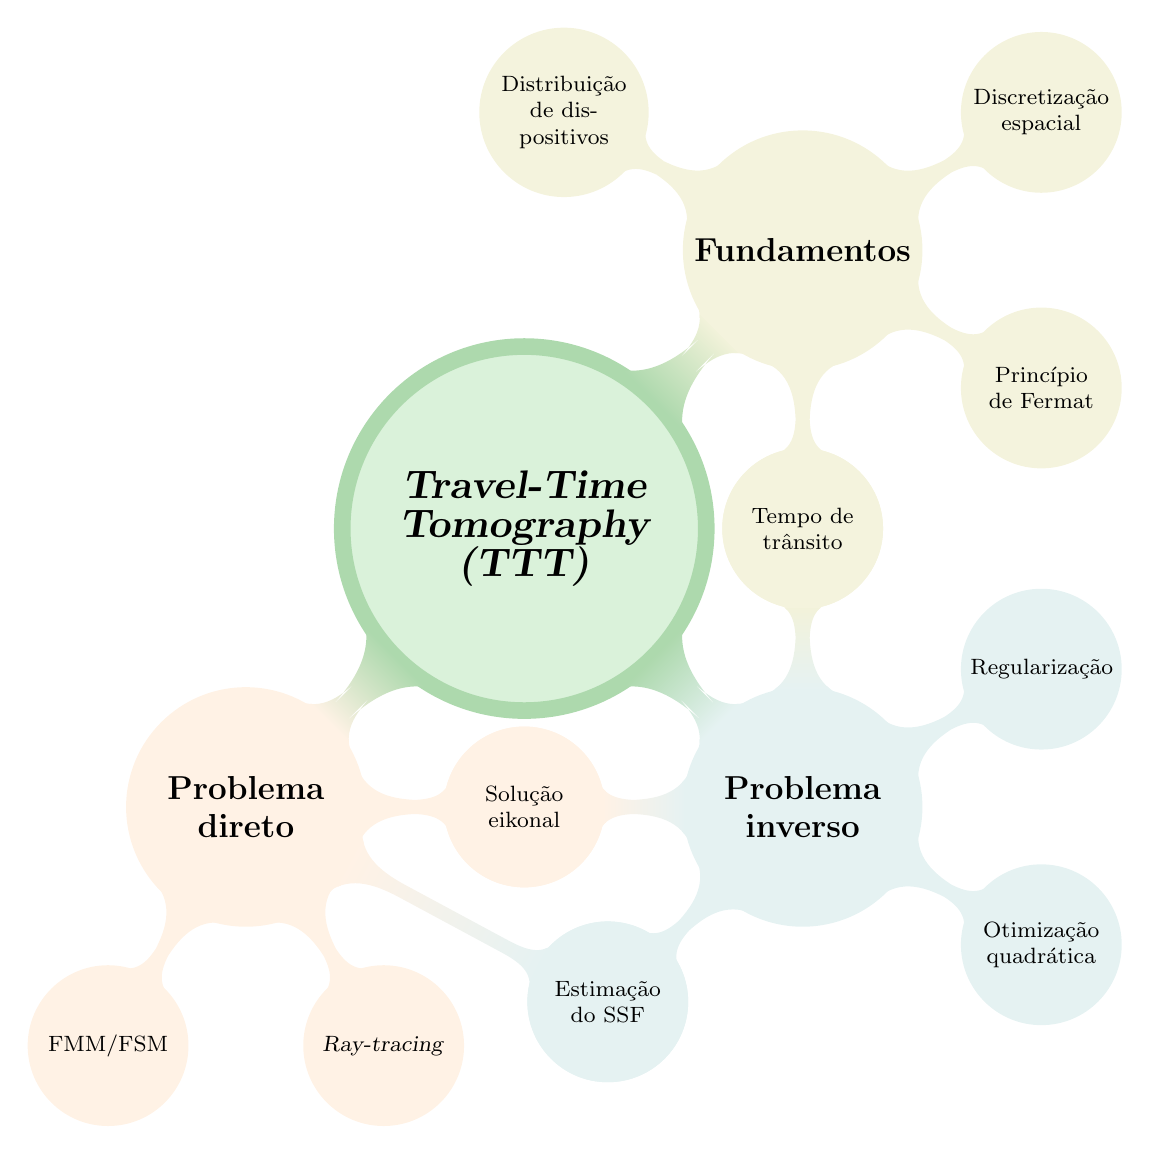
\begin{tikzpicture}[
			mindmap,
			text width=2.5cm,
			align=center,
			every node/.style={concept},
			concept color=green!20!white!85!black,
			level 1/.append style={
				level distance=5cm,
				minimum size=3cm,
				text width=2.8cm,
				font=\large,
			},
			level 2/.append style={
				level distance=3.5cm,
				minimum size=2cm,
				text width=1.8cm
			},
			]
			
			\node[minimum size=4.5cm, text width=4.3cm, line width=6pt, fill=green!10!white!95!black] (TTT) {\Large\textbf{\textsl{Travel-Time \mbox{Tomography} (TTT)}}}
			child[concept color=yellow!10!white!95!black,grow=45] { 
				node (fundamentos) {\textbf{Fundamentos}}
				child[grow=150] { node{Distribuição\\de dispositivos} }
				child[grow=30] { node{Discretização\\espacial} }
				child[grow=-30] { node{Princípio\\de Fermat} }
				child[grow=-90] { node (tt) at (fundamentos|-TTT) {Tempo de\\trânsito} }
			}
			child[concept color=teal!10,grow=315] { 
				node (probinv) {\textbf{Problema\\inverso}}				
				child[grow=-30] { node{Otimização\\quadrática} }
				child[grow=30] { node{Regularização} }
				child[concept color=yellow!10!white!95!black] { node at (tt) {Tempo de trânsito}}
				child[concept color=orange!10] { node (solucaoeikonal) at (TTT|-probinv) {Solução\\eikonal} }
				child[grow=225] { node (estimssf) {Estimação\\do SSF} }
			}
			child[concept color=orange!10,grow=225] { 
				node (probdir) {\textbf{Problema\\direto}} 
				child[grow=300] { node{\textsl{Ray-tracing}} }
				child[grow=240] { node{FMM/FSM} }
				child { node at (solucaoeikonal) {Solução\\eikonal} }
				child[concept color=teal!10] { node at (estimssf) {Estimação\\do SSF} }
%				child[concept color=teal!10,grow=315, level distance=5cm] { node(estssf) {} }
			}
			;	
	\end{tikzpicture}
	\caption[\textsl{Mindmap} da \cref{sec:travel-time_tomography}.]{\textsl{Mindmap} da \cref{sec:travel-time_tomography} sobre a tomografia de tempo de trânsito.}
	\label{fig:mindmap_sec2}
\end{figure}


	\section{Inversão utilizando tempo de trânsito}
\label{sec_rt}
Seguindo as ideias da revisão bibliográfica anterior, foi realizada uma segunda pesquisa. Nela, o objetivo é buscar artigos que tratem do problema de inversão tomográfica utilizando primariamente informação de tempo de trânsito, mas não se atendo obrigatoriamente à técnica de \gls{ttt}.

Nesta revisão, focamos em uma seleção de periódicos (\quote{IEEE Trans. on Instrumentation and Measurement}, \quote{IEEE Trans. on Geoscience and Remote Sensing}, e \quote{IEEE Journal of Oceanic Engineering}) e termos (\quote{Acoustic Tomography}, \quote{Travel Time Tomography}, e \quote{Seismic Tomography}). Um total de 47 artigos foram extraídos dos primeiros 125 resultantes da busca no IEEExplore, dos quais 17 foram posteriormente selecionados por estarem relacionados à tomografia com tempo de trânsito (não especificamente \ingles{Travel-Time Tomography}), e 4 foram finalmente filtrados por possuírem reflexões mais profundas ou detalhadas que melhor se adequam à pesquisa atual.

\subsection{Leitura superficial nos artigos selecionados}

Aqui falaremos brevemente sobre cada artigo selecionado, destacando (citação em negrito) os mais promissores, com abordagens e desenvolvimentos teóricos que poderiam ser úteis.

\begin{itemize}
	\citem{agata_bayesian_2023} - Utiliza \gls[PINNs][redes neurais fisicamente informadas][Physically-Informed Neural Networks]{pinn} treinadas para resolver a equação eikonal e estimar o \gls{ssf}.
	\citem{bao_online_2020} - Adiciona um termo de regularização temporal na função de custo para utilizar informações de tempo de trânsito de múltiplas janelas.
	\citem{carriere_featureoriented_2013} - Usa tomografia acústica para estimação de perfil de temperatura em corpo d'água.
	\citem{djikpesse_reducing_2010} - Utiliza modelos \gls{ttt} para estimar e corrigir perfis de velocidade ao longo de poços.
	\citem{goyal_ultrasound_2025} - Utiliza modelos \gls{ttt} para reconstruir imagens pulmonares.
	\citem{gras_practical_2022} - Utiliza modelos \gls{ttt} para reconstrução de estruturas de velocidade de onda P subsuperficiais. Refina adicionalmente este modelo usando \gls{fwi}.
	\citem{han_realtime_2014} - Foca no desenvolvimento de um sistema de imageamento 3D na água em tempo-real usando \ingles{beamforming}, mas parece não considerar \ingles{raybending}.
	\citem{jo_seismic_2023,jo_seismic_2024} - Ambos os artigos utilizam \gls[NNs][redes neurais][Neural Networks]{nn} para TTT, usando diferentes abordagens de \gls{ml} para o treinamento da \gls{nn}.
	\citem{li_multiscale_2024} - Utiliza múltiplas grades deslocadas para alcançar complementarmente resultados mais precisos na inversão de velocidade sísmica. Não utiliza \gls{ttt}, embora utilize informações de tempo de trânsito.
	\citem{mei_uncertainty_2025} - Implementa \gls{ttt} através de \gls[NNs]{nn} e desenvolve novas abordagens de quantificação de incerteza.
	\citem{othmani_acoustic_2024} - Utiliza \gls{ttt} e dados de tempo de trânsito para reconstrução de campos de temperatura interna.
	\citem{shin_distributed_2022} - Minimiza a função de custo \gls{ttt} sujeita à equação eikonal, em vez de resolver ambas iterativamente.
	\citem{wang_seismic_2024} - Muito semelhante a \cite{jo_seismic_2023}, usando uma abordagem de ML diferente para o treinamento.
	\citem{wo_firstarrival_2024} - Utiliza uma estrutura \gls{ttt} ligeiramente modificada (força a função de regularização a ser 0 em vez de adicioná-la à minimização) e adiciona informações da estrutura à função-custo.
	\citem{yu_krylov_2021} - Emprega métodos de subespaço de Krylov para lidar com o problema mal posto de TTT, inversão acústica e reconstrução de campos de velocidade do som.
	\citem{yu_review_2022} - Um artigo de revisão sobre o uso de informações de tempo de trânsito na reconstrução de campos de velocidade do som e temperatura, através de diferentes técnicas e abordagens.
	\citem{zhang_optimization_2023} - Estuda a otimização do arranjo de transdutores (dispositivos), para reconstrução de SSF com \gls{ttt}, considerando também o fluxo de fluido.
	\citem{zhang_nonlinear_2022} - Utiliza \gls{ttt} para estimação do \gls{ssf} e propõe/destaca uma nova abordagem de \textsl{ray-tracing}.
\end{itemize}

\subsection{Análise aprofundada}
\label{sec_rt:subsec_deeper-analysis}

Dada a leitura superficial anterior dos artigos e a eleição de alguns que estão mais alinhados com as necessidades da pesquisa atual, estes selecionados serão agora apresentados e discutidos mais profundamente.

\papersec{\citeay*{li_multiscale_2024}}

O objetivo deste artigo de \cite{li_multiscale_2024} é o mesmo do projeto --- inversão de campo de velocidade através de tomografia sísmica --- embora focado na estimativa de estrutura de subsuperfície, em vez da modelagem do \gls{ssf}. No lugar da tradicional minimização do erro de tempo de trânsito sujeita a uma restrição de regularização, a abordagem deles minimiza o erro da equação eikonal, sujeita a uma restrição de tempo nulo de percurso nas fontes\footnote{O problema deles separa entre ondas fonte-receptor e ondas receptor-fonte, cada uma com tempo $0$ na sua origem.}. Esta técnica é chamada de \quote{\ingles{Fixed-scale regular-grid adjoint-state First-Arrival Slope Tomography seismic velocity inversion method}} (ou FFAST).

Expandindo isso, eles propuseram um \quote{Multiscale FFAST} (ou MFAST), utilizando múltiplas grades com diferentes escalas e deslocamentos, estimando o SSF modelado em cada uma, e usando uma interpolação cubic spline para fundir as diferentes estimativas e alcançar uma solução global. Seus resultados comparam o FAT (\gls{ttt} tradicional, como exposto anteriormente), FFAST e MFAST, mostrando que as abordagens FFAST e o MFAST proposto tiveram resultados melhores (embora marginalmente).

\begin{itemize}
	\item Múltiplas grades com diferentes espaçamentos (\textsl{Multiscale})
	\item Uso do esquema de minimização FFAST em vez de \gls{ttt} - função de custo diferente
	\item Não necessita de um resolvedor eikonal, dado o esquema de minimização
\end{itemize}

\papersec{\citeay*{shin_distributed_2022}}

Neste artigo \cite{shin_distributed_2022}, eles usam uma estrutura baseada em \gls{ttt}, minimizando o erro de tempo de trânsito sujeito à equação eikonal (esta sujeita a tempo de trânsito zero na fonte), em vez da tradicional minimização alternada de cada um. Semelhante a \cite{li_multiscale_2024}, uma abordagem de \textsl{adjoint state} é empregada, fundindo a restrição da equação eikonal na função custo. O método FSM é usado para resolver a etapa da equação eikonal. Então, uma solução para o modelo de vagarosidade (\textsl{slowness}) é atualizada iterativamente, até que a convergência seja alcançada.

Além disso, o trabalho deles propõe uma \gls{ttt} distribuída, onde um subconjunto de toda a informação de tempo de trânsito (ou uma aproximação da informação) está disponível em cada nó (receptor), e cada receptor atualiza localmente seu modelo. Isso é relevante para sistemas não centralizados, o que não se aplica ao cenário atual, onde toda a informação é reunida em uma unidade central de processamento encarregada de estimar o \gls{ssf}. No entanto, o esquema de minimização empregado neste artigo pode ser útil e aplicável na pesquisa atual.

\begin{itemize}
	\item Função de custo diferente quando comparada ao \gls{ttt}
	\item Usa um esquema computacional distribuído, em vez do tradicional centralizado
	\item Usa o FSM, que poderia ser substituído por \gls{fmm}
\end{itemize}

\papersec{\citeay*{yu_krylov_2021}}

Neste artigo \cite{yu_krylov_2021}, em vez de estimar a vagarosidade (e, portanto, a velocidade) em cada célula, eles tratam o perfil de vagarosidade como uma função-vetor sobre um espaço determinado por uma base de funções de \textsl{kernel}, com suas respectivas entradas vetoriais sendo os parâmetros sobre esta base, sendo estes os valores estimados no processo de minimização. O problema inicial deles é a otimização \gls{ttt} básica, usando uma regularização RMS em vez de uma de suavidade (Laplaciano espacial discreto).

Eles comparam diferentes bases de \textsl{kernel} e diferentes subespaços de Krylov para resolver o processo de minimização para alguns modelos de temperatura.

\begin{itemize}
	\item Usa um espaço de minimização totalmente diferente, mas ainda baseado no \gls{ttt}
	\item Explora diferentes subespaços e bases de funções
\end{itemize}

\papersec{\citeay*{zhang_nonlinear_2022}}

Neste artigo \cite{zhang_nonlinear_2022}, eles usam um algoritmo evolutivo para encontrar a solução ótima para o campo de vagarosidade, em vez de um problema de minimização iterativo baseado em gradiente. Eles também consideram um campo de velocidade de fluxo junto com o campo de velocidade estático, e trazem um novo método de \textsl{ray-tracing} baseado na otimização de três pontos das curvas. Este algoritmo de \textsl{ray-tracing} aproxima o raio como uma sequência de pontos e atualiza iterativamente essas posições perturbando sistematicamente a posição de cada ponto com base em seus vizinhos e no campo de rapidez/velocidade.

Tendo os raios, uma nova geração de possíveis candidatos é gerada com base na média ponderada da geração anterior e outros parâmetros estáticos e dinâmicos. As vantagens desta abordagem residem na sua independência de um cálculo de gradiente, que pode ser computacionalmente dispendioso.

\begin{itemize}
	\item Usa um algoritmo evolutivo em vez de um baseado em gradiente para otimizar o \gls{ssf}
	\item Usa um algoritmo de \textsl{ray-tracing} proposto em vez de um resolvedor eikonal
\end{itemize}

\subsection{\textsl{Mindmap} e conclusões}

A \cref{fig:mindmap_sec3} apresenta um \textsl{mindmap} resumindo a revisão dos artigos apresentados em relação aos métodos utilizados, às aplicações, e aos tipos de dados de entrada que cada artigo utiliza. O número em cada nó menor é a quantidade de artigos que se encaixa naquela classificação. Essas classificações serão revisitadas e expandidas na \cref{sec:cp}.

Dada a natureza dessa revisão bibliográfica, a esmagadora maioria dos artigos utiliza informação de tempo de trânsito. No método, uma boa parte utiliza métodos derivados da formulação de \gls{ttt}, alguns utilizam os dados de tempo de trânsito como entrada para treinamento de redes neurais, e alguns outros propõem formulações diferentes. Quanto à aplicação, a maior parte restringe-se ao imageamento de estruturas geológicas, com alguns tratando da estimação de perfis de temperatura em ambientes.
%\section{Mindmap}
%\vfill
\begin{figure}[!t]
	\centering
	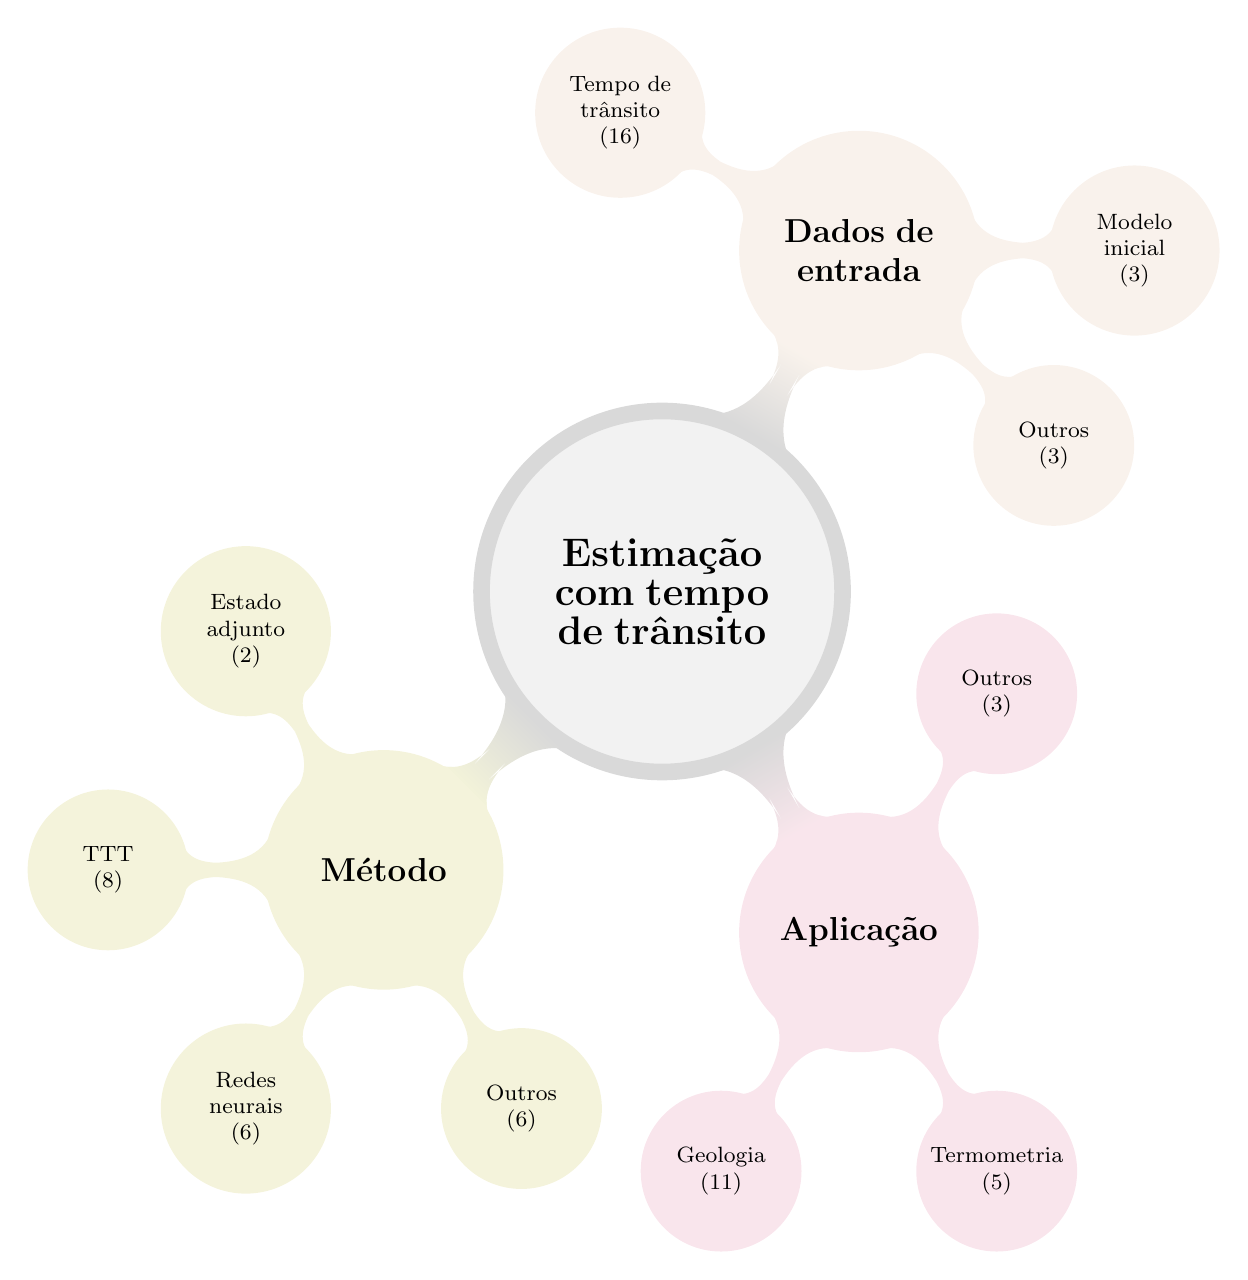
\begin{tikzpicture}[
			mindmap,
			text width=2.5cm,
			align=center,
			every node/.style={concept},
			concept color=gray!30,
			level 1/.append style={
				level distance=5cm,
				minimum size=3cm,
				text width=2.8cm,
				font=\large,
			},
			level 2/.append style={
				level distance=3.5cm,
				minimum size=2cm,
				text width=1.8cm
			},
			]
			
			\node[minimum size=4.5cm, text width=4.3cm, line width=6pt, fill=gray!10] (TTT) { \Large\textbf{Estimação com tempo de trânsito} }
			child[concept color=olive!10,grow=225] { 
				node {\textbf{Método}} 
				child[grow=120] { node {Estado adjunto \\(2)} }
				child[grow=180] { node {TTT \\(8)} }
				child[grow=240] { node {Redes neurais \\(6)} }
				child[grow=300] { node {Outros \\(6)} }
			}
			child[concept color=purple!10, grow=300] {
				node {\textbf{Aplicação}}
				child[grow=240] { node {Geologia \\(11)} }
				child[grow=300] { node {Termometria \\(5)} }
				child[grow=60] {node {Outros \\(3)} }
			}
			child[concept color=brown!10, grow=60] {
				node {\textbf{Dados de entrada}} 
				child[grow=150] { node {Tempo de trânsito \\(16)} }
				child[grow=0] { node {Modelo inicial \\(3)} }
				child[grow=-45] { node {Outros \\(3)}}
			}
			;	
	\end{tikzpicture}
	\caption[\textsl{Mindmap} da \cref{sec_rt}]{\textsl{Mindmap} da \cref{sec_rt} sobre inversão com tempo de trânsito.}
	\label{fig:mindmap_sec3}
\end{figure}
	\section{Revisão bibliográfica da inversão de SSF/SSP na coluna d'água}
\label{sec_rssfi}
Como também sugerido em reuniões, outra revisão foi conduzida, agora buscando na literatura ferramentas tecnológicas e matemáticas dentro da inversão da velocidade do som na coluna d'água. Especificamente, buscamos diferentes abordagens para o problema de alocação de dispositivos que surge ao lidar com águas profundas, diferentes tipos de informação --- e, portanto, diferentes técnicas --- que são usadas nesta inversão, e outros insights que possam ser úteis e importantes neste cenário. Nesta revisão, uma busca geral foi feita no Google Scholar, procurando pelo termo \quote{\textsl{water column velocity inversion}}. Dos primeiros (mais relevantes) 100 artigos da busca no Google Scholar, 30 foram pré-selecionados por terem potencial e, destes, 7 foram selecionados por estarem relacionados à pesquisa atual.

\subsection{Leitura superficial nos artigos selecionados}

\begin{itemize}
	\citem{abakumov_timelapse_2019} - Artigo raso demais para extrair qualquer informação útil.
	\citem{amini_joint_2016} - Usa/corrobora a noção de que, abaixo de uma certa profundidade (aqui assumida como $z_0 = 1250\si{\meter}$), um modelo externo pode ser usado. Também estima conjuntamente o SSF e corrige o posicionamento dos nós.
	\citem{ashley_inverted_1998} - Usa Ecobatímetros Invertidos (Inverted Echo Sounders) para estimar a espessura das camadas de água no Ártico. Não aborda a etapa de inversão.
	\citem{becker_geoacoustic_2007} - Foca na inversão geoacústica para batimetria do assoalho oceânico. Não aborda a etapa de inversão.
	\citem*{bender_threedimensional_2012} - Foca na inversão 3D de SSF na coluna d'água. Pode ser útil. Tese.
	\citem{chapeland_highresolution_2022} - Usa FWI e JMI para modelagem de estrutura de subsuperfície.
	\citem{cvetkovic_inverting_2019} - Artigo raso demais para extrair qualquer informação útil.
	\citem{datta_fast_2019} - Usa uma FWI adaptada para separar o campo estático (água) do campo dinâmico (subsuperfície), para estimar a estrutura da porção dinâmica.
	\citem{deluca_simultaneous_2022} - Emprega FWI para inversão de subsuperfície em águas rasas.
	\citem*{dosso_joint_2023} - Usa inversão estatística (Bayesiana) para estimar conjuntamente as estruturas de velocidade da coluna d'água e da subsuperfície. Pode ser relevante.
	\citem{fortin_extracting_2015} - Estima turbulência oceânica, usa \ingles{prestacking FWI} para imageamento de subsuperfície, e alguns outros estudos. Não parece relacionado.
	\citem{hou_velocity_2018} - Estima separadamente a coluna d'água (rasa) e o solo próximo à superfície, usando outros dados (temperatura, salinidade) para a porção da coluna d'água. Não detalha os processos de inversão.
	\citem{lacasse_water_2011} - Estuda os efeitos de fontes de erros sistemáticos (erro de posicionamento e efeitos do SSF) na aquisição de dados e inversão. Não estuda a inversão de SSF.
%	\citem{lecerf_water_2022} - Ainda não entendo qual é o objetivo deles ou o que eles estão realmente fazendo.
	\citem{lin_equivalent_2006} - Quantifica discrepâncias no SSF e estuda seus efeitos na inversão geoacústica.
	\citem{mallick_prediction_2022} - Propõe uma nova inversão de forma de onda para gerar modelos iniciais para estimativa de SSF e, posteriormente, para estimativa de parâmetros (temperatura e salinidade).
	\citem{mcmechan_application_1982} - Verifica o uso do método de \ingles{downward contribuition} para abordar a inversão sísmica usando dados de refração.
	\citem{michalopoulou_environmental_2018} - Usa rastreamento de dispersão e análise modal para estimativa de profundidade da coluna d'água e inversão sísmica.
	\citem{mitchell_optical_2018} - Estima propriedades ópticas em um corpo d'água dadas as propriedades do campo de luz espectral medidas por \ingles{gliders}.
	\citem*{radhakrishnan_inversion_2024} - Estima o SSF na água usando informações de tempo de percurso para situações de águas rasas, usando funções empíricas como base.
	\citem*{ritter_water_2010} - Usa dados de tempo de percurso para inversão de SSF, assumindo o conhecimento de um modelo/estado anterior para o perfil de velocidade.
	\citem{takeuchi_development_1993} - Visa modelar correntes de água usando ondas que viajam em direções opostas dentro do corpo d'água.
	\citem{taroudakis_tomographic_2001} - Usa informações de tempo de percurso para inversão tomográfica em águas rasas, usando modelagem modal do SSF.
	\citem{vadapalli_application_2012} - Muito semelhante a \cite{ritter_water_2010}.
	\citem*{voort_inversion_2022} - Propõe dois modelos inovadores para inversão de SSF considerando informações não confiáveis/inacessíveis sobre o posicionamento dos dispositivos. Tese.
	\citem{wellington_2d_2015} - Usa FWI em domínio do tempo de banda larga para inversão acústica.
	\citem{wong_leastsquares_2011} - Apresenta um estudo de caso para o uso de RTM para imageamento de estruturas de solo em subsuperfície.
	\citem*{wu_inversion_2023} - Usa informações de tempo de percurso e tomografia acústica para estimativa dos parâmetros do perfil de Munk, usando isso como um esquema de inversão de SSP.
	\citem{zhang_inversion_2016} - Usa \ingles{acoustic field matching} para estimativa de SSF usando ROVs.
\end{itemize}

\subsection{Análise aprofundada}
\label{sec_rssfi:subsec_deeper-analysis}

Tendo a leitura superficial anterior e, com ela, a seleção de artigos mais relevantes, estes serão agora analisados e apresentados de forma mais completa.

\papersec{\citeay*{bender_threedimensional_2012}}

Esta tese \cite{bender_threedimensional_2012} desenvolve um novo esquema de inversão para inversão de SSFs 3D em cenários de coluna d'água. Baseia-se em uma abordagem linearizada e modela a perturbação em relação a um cenário de base, e na \quote{equação de modo normal separada por profundidade}, uma EDO não linear de segunda ordem. Utiliza um esquema de minimização diferente baseado em equações de modo normal, empregando informações derivadas do tempo de percurso para o processo de inversão. A tese também é muito extensa e exigiria uma leitura ainda mais profunda e lenta.

\papersec{\citeay*{dosso_joint_2023}}

Este artigo \cite{dosso_joint_2023} utiliza inversão estatística e Bayesiana de dados acústicos para reconstrução conjunta do SSF e do modelo geoacústico do leito marinho. Utiliza formas de onda acústicas como informação de entrada para a inversão, sendo, portanto, incompatível (em sua forma atual) com a inversão baseada em tempo de percurso desejada. Algumas outras suposições (como a linearidade da velocidade do som entre os nós) também são adotadas.

\begin{itemize}
	\item Considera a profundidade do fundo do mar desconhecida, a posição dos nós e os parâmetros (dos nós) a serem estimados
	\item Parece assumir verticalidade entre os dispositivos
	\begin{itemize}
		\item Ignora o movimento transversal (horizontal)
		\item Ignora \ingles{ray bending}
		\item Não requer um solver Eikonal
	\end{itemize}
	\item Utiliza informações de forma de onda acústica (indisponíveis para nós)
\end{itemize}

\papersec{\citeay*{radhakrishnan_inversion_2024}}

Aqui \cite{radhakrishnan_inversion_2024}, eles propõem o uso de funções ortogonais empíricas (EOFs) como base, com as quais o SSF objetivo invertido é uma combinação linear ao longo desta base. Eles usam informações de tempo de percurso de múltiplos caminhos (multipath) em relação aos sinais (o que requer pelo menos algum nível de gravação acústica) para estimar a resposta ao impulso do canal e, a partir disso, inverter o SSF. Finalmente, eles usam essas possíveis soluções geradas por EOF para alimentar um algoritmo evolutivo, que refinará a saída.

\papersec{\citeay*{ritter_water_2010}}

Neste artigo \cite{ritter_water_2010}, o problema tratado é muito semelhante ao TTT tradicional, mas estimando iterativamente uma perturbação a ser aplicada a um modelo anterior (ou inicial). Eles também consideram uma posição vertical variável dos refletores (considerando uma comunicação ROV-OBN-ROV), e integram a estimação da posição vertical à minimização. Outras simplificações são adotadas, como a suposição de uma velocidade constante no ROV.

\papersec{\citeay*{wu_inversion_2023}}

Neste artigo \cite{wu_inversion_2023}, em vez de estimar o SSF em cada ponto/célula de forma \quote{independente} (sujeito à regularização e interação com outras células), propõe-se usar o perfil de Munk como diretriz, e a estimativa é feita sobre os parâmetros do perfil. Eles também consideram uma topografia do leito marinho não suave, levando em conta diferentes formas e sua interação com as ondas em propagação.

Não está claro se o artigo considera um ambiente 3D ou apenas uma variação 1D --- trabalhando sob uma suposição estratificada (cada profundidade tem a mesma velocidade) --- em seu desenvolvimento matemático, mas mesmo no último caso ainda seria viável aplicá-lo a um ambiente 3D, adaptando a formulação.

%\subsection{Considerações práticas}
%
%Dos artigos lidos, encontramos algumas abordagens diferentes, desde o uso de informações completas da forma de onda (e, assim, empregando FWI ou outras técnicas semelhantes), até diferentes abordagens de modelagem (paramétrica em vez de inversão direta). Diferentes problemas também foram tratados e, embora a maioria possa ser adaptada para o cenário 3D que está sendo estudado, alguns são inerentemente unidimensionais e, portanto, incompatíveis com o problema em questão.
%
%Entre os artigos escolhidos, \cite{bender_threedimensional_2012} é interessante, pois utiliza informações de tempo de percurso, mas a partir de um ponto de partida muito diferente. \cite{wu_inversion_2023} também pode ser útil, pois eles otimizam os parâmetros do perfil de Munk para se ajustarem aos dados adquiridos, o que poderia ser proveitoso, especialmente em ambientes mais profundos.
%
%Estes artigos, aliados aos apresentados na \cref{sec_rt}, poderiam ajudar a desenvolver uma nova técnica matemática capaz de lidar com o problema em questão, que já se mostrou (em outros documentos) insolúvel apenas com a técnica de TTT, sem novos desenvolvimentos práticos consideráveis e/ou uso de informações (atualmente não disponíveis) sobre pressão, temperatura e salinidade, ou de caras expedições de ROV ao longo do perfil vertical.

%\section{Mindmap}
%\vfill
\begin{figure}[!t]
	\centering
	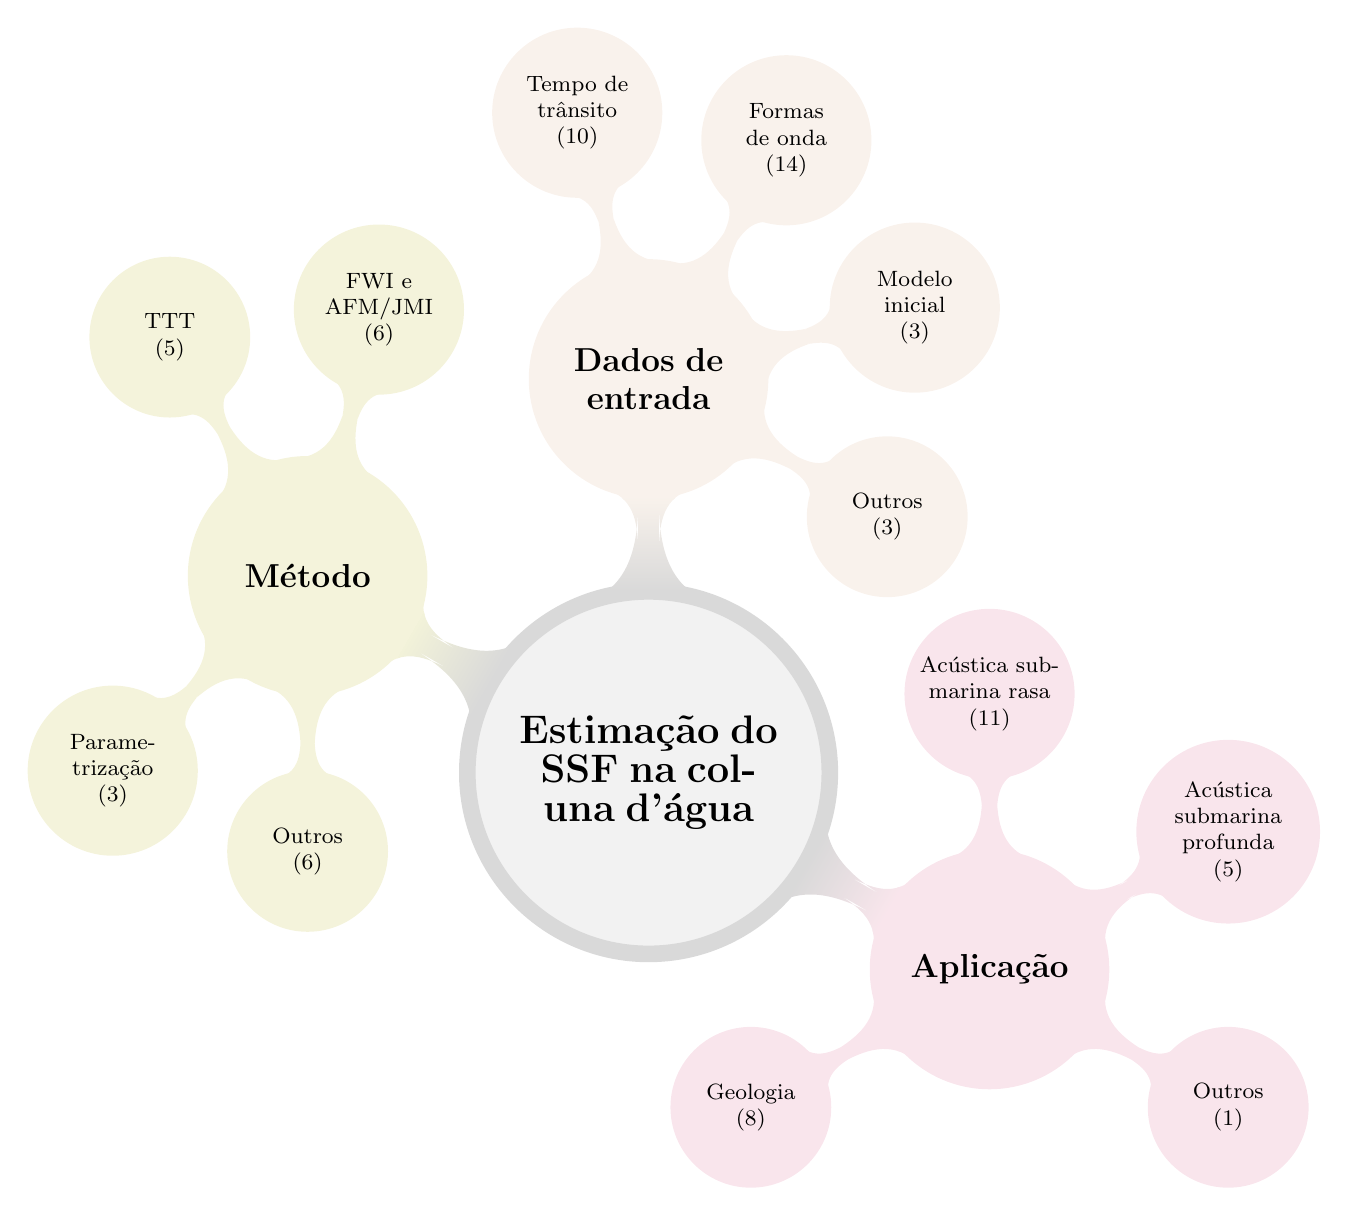
\begin{tikzpicture}[
		mindmap,
		text width=2.5cm,
		align=center,
		every node/.style={concept},
		concept color=gray!30,
		level 1/.append style={
			level distance=5cm,
			minimum size=3cm,
			text width=2.8cm,
			font=\large,
		},
		level 2/.append style={
			level distance=3.5cm,
			minimum size=2cm,
			text width=1.8cm
		},
		]
		
		\node[minimum size=4.5cm, text width=4.3cm, line width=6pt, fill=gray!10] (TTT) { \Large\textbf{Estimação do SSF na coluna d'água} }
		child[concept color=olive!10,grow=150] { 
			node {\textbf{Método}} 
			child[grow=75] { node {FWI e AFM/JMI \\(6)} }
			child[grow=120] { node {TTT \\(5)} }
			child[grow=225] { node {Parame\-trização \\(3)} }
			child[grow=270] { node {Outros \\(6)} }
		}
		child[concept color=purple!10, grow=330] {
			node {\textbf{Aplicação}}
			child[grow=90] { node {Acústica submarina rasa \\(11)} }
			child[grow=30] { node {Acústica submarina profunda \\(5)} }
			child[grow=210] { node {Geologia \\(8)} }
			child[grow=330] {node {Outros \\(1)} }
		}
		child[concept color=brown!10, grow=90] {
			node {\textbf{Dados de entrada}} 
			child[grow=105] { node {Tempo de trânsito \\(10)} }
			child[grow=60] { node {Formas de onda \\(14)} }
			child[grow=15] { node {Modelo inicial \\(3)} }
			child[grow=-30] { node {Outros \\(3)}}
		}
		;	
	\end{tikzpicture}
	\caption{\textsl{Mindmap} da \cref{sec_rssfi}.}
	\label{fig:mindmap_sec4}
\end{figure}

\subsection{\textsl{Mindmap} e conclusões}

A \cref{fig:mindmap_sec4} mostra um \textsl{mindmap} resumindo a revisão dos artigos apresentados em relação aos métodos utilizados, às aplicações, e aos tipos de dados de entrada que cada artigo utiliza. Novamente, o número em cada nó indica a quantidade de artigos relacionados, com essas classificações sendo revisitadas e mais profundamente detalhadas na \cref{sec:cp}.

Dada a liberdade quanto ao método de inversão dos artigos selecionados nessa revisão, uma boa parte deles utilizou informações de forma de onda do sinal, e não somente tempo de trânsito, como o dado adquirido nos receptores. Em função disso, uma boa parte dos artigos também realizou inversões baseadas em dados de forma de onda (como FWI, AFM, e JMI). Interessantemente, mesmo com dados de tempo de trânsito disponíveis, poucos realizaram inversão baseada diretamente na TTT. Além disso, a aplicação de uma boa parte deles se restringia à acústica submarina rasa (até $\sim500\si{\meter}$) e à geologia, com poucas aplicações na acústica submarina profunda. Não está claro se esse escopo de aplicação se deve a limitações do método, ou não-aplicação dos resultados à estimação de campos de velocidade em grandes profundidades.
	\section{Análise comparativa entre os artigos revisados}
\label{sec:cp}

Nessa seção serão comparados os artigos apresentados nas \cref{sec_rt,sec_rssfi}, classificando-os quanto a algumas características de interesse deles, e buscando estabelecer possíveis frentes para pesquisa e métodos de interesse, que se encaixem no escopo do projeto. Aqui não serão discutidos ou reapresentados os artigos da \cref{sec:travel-time_tomography}, dado que os artigos lá mostrados são muito semelhantes entre si, e é possível descrever a \gls{ttt} através deles.

\subsection{Classificação dos artigos/técnicas}
\label{subsec:cp_classif}

Todos os artigos revisados (não somente os destacados) serão classificados, conforme as características dos métodos propostos e empregados, tipos de dados usados, entre outras categorias. Todos os artigos\footnote{Os artigos da \cref{sec_rt} estarão em azul, os da \cref{sec_rssfi} em vermelho; os artigos selecionados de cada seção estarão em negrito.} serão caracterizados pelas seguintes informações:
\begin{enumerate}[itemsep=-1ex, partopsep=0pt]
	\item Abordagem ou método (modelo direto, funções-base, parametrização, \textit{machine learning})
	\item Dimensão da aplicação (1D$\sim$4D)
	\item Aplicação (acústica submarina rasa, acústica submarina profunda, estruturas geológicas, biomédica)
	\item Dados de entrada (tempo de trânsito, forma de onda, modelo inicial)
	\item Parâmetros ajustáveis (vagarosidade, pesos de funções-base, parâmetros)
	\item Métrica de erro ou método de avaliação
\end{enumerate}

\begingroup
\definecolor{tomographycolor}{RGB}{0, 0, 255}
\definecolor{ssfinvcolor}{RGB}{255, 0, 0}

\renewcommand{\arraystretch}{1.5}

\begin{table}[H]
	\def\seleccite{\bfseries}
	\centering
	\caption{Abordagem ou método}
	\label{table:cp_classif_metodo}
	\begin{tabular}{C{0.3\linewidth} C{0.5\linewidth}}
		\textbf{Características} & \textbf{Trabalhos} \\
		\ttline
		%		\vphantom{\rule{0.4pt}{1.2em}}
		TTT & 
		\cite{bao_online_2020}
		\cite{djikpesse_reducing_2010}
		\cite{goyal_ultrasound_2025}
		\cite{gras_practical_2022}
		\cite{othmani_acoustic_2024}
		\cite{shin_distributed_2022}
		\cite{wo_firstarrival_2024}
		\cite{zhang_optimization_2023}
		\cite{mcmechan_application_1982}
		\cite{ritter_water_2010}
		\cite{takeuchi_development_1993}
		\cite{vadapalli_application_2012}
		\cite{wellington_2d_2015}
		\\\tline
		Outros modelos diretos &
		\cite{gras_practical_2022}
		\cite{li_multiscale_2024}
		\cite{chapeland_highresolution_2022}
		\cite{datta_fast_2019}
		\cite{deluca_simultaneous_2022}
		\cite{mallick_prediction_2022}
		\cite{michalopoulou_environmental_2018}
		\cite{wong_leastsquares_2011} 
		\cite{zhang_inversion_2016}
		\\\tline
		Modelagem estatística &
		\cite{agata_bayesian_2023}
		\cite{dosso_joint_2023}
		\\\tline
		Funções-base &
		\cite{yu_krylov_2021}
		\cite{radhakrishnan_inversion_2024}
		\cite{taroudakis_tomographic_2001}
		\\\tline
		Parametrização &  
		\cite{carriere_featureoriented_2013}
		\cite{wu_inversion_2023}
		\\\tline
		\textit{Machine Learning} &
		\cite{agata_bayesian_2023}
		\cite{jo_seismic_2023}
		\cite{jo_seismic_2024}
		\cite{mei_uncertainty_2025}
		\cite{wang_seismic_2024} 
		\cite{zhang_nonlinear_2022}
		\cite{mallick_prediction_2022}
		\\\tline
		Outros & 
		\cite{han_realtime_2014}
		\cite{amini_joint_2016}
		\cite{ashley_inverted_1998}
		\cite{becker_geoacoustic_2007}
		\cite{bender_threedimensional_2012}
		\cite{mitchell_optical_2018}
	\end{tabular}
\end{table}

\begin{table}[H]
	\def\seleccite{\bfseries}
	\centering
	\caption{Dimensão da aplicação}
	\begin{tabular}{C{0.3\linewidth} C{0.5\linewidth}}
		\textbf{Características} & \textbf{Trabalhos} \\
		\ttline
		1D & 
		\cite{carriere_featureoriented_2013}
		\cite{djikpesse_reducing_2010}
		\cite{amini_joint_2016}
		\cite{dosso_joint_2023}
		\\\tline
		2D, 3D, ou 4D &
		\cite{agata_bayesian_2023}
		\cite{bao_online_2020}
		\cite{goyal_ultrasound_2025}
		\cite{gras_practical_2022}
		\cite{han_realtime_2014}
		\cite{jo_seismic_2023}
		\cite{jo_seismic_2024}
		\cite{li_multiscale_2024}
		\cite{mei_uncertainty_2025}
		\cite{othmani_acoustic_2024}
		\cite{shin_distributed_2022}
		\cite{wang_seismic_2024}
		\cite{wo_firstarrival_2024}
		\cite{yu_krylov_2021}
		\cite{zhang_optimization_2023}
		\cite{zhang_nonlinear_2022}
		\cite{bender_threedimensional_2012}
		\cite{chapeland_highresolution_2022}
		\cite{datta_fast_2019}
		\cite{deluca_simultaneous_2022}
		\cite{hou_velocity_2018}
		\cite{lin_equivalent_2006}
		\cite{mallick_prediction_2022}
		\cite{mcmechan_application_1982}
		\cite{michalopoulou_environmental_2018}
		\cite{mitchell_optical_2018}
		\cite{radhakrishnan_inversion_2024}
		\cite{ritter_water_2010}
		\cite{takeuchi_development_1993}
		\cite{taroudakis_tomographic_2001}
		\cite{vadapalli_application_2012}
		\cite{voort_inversion_2022}
		\cite{wellington_2d_2015}
		\cite{wong_leastsquares_2011}
		\cite{wu_inversion_2023}
		\cite{zhang_inversion_2016}
	\end{tabular}
\end{table}

\begin{table}[H]
	\def\seleccite{\bfseries}
	\centering
	\caption{Aplicação}
	\label{table:cp_classif_aplicacao}
	\begin{tabular}{C{0.3\linewidth} C{0.5\linewidth}}
		\textbf{Características} & \textbf{Trabalhos} \\
		\ttline
		Acústica submarina rasa & 
		\cite{abakumov_timelapse_2019}
		\cite{amini_joint_2016}
		\cite{deluca_simultaneous_2022}
		\cite{dosso_joint_2023}
		\cite{hou_velocity_2018}
		\cite{mallick_prediction_2022}
		\cite{radhakrishnan_inversion_2024}
		\cite{taroudakis_tomographic_2001}
		\cite{voort_inversion_2022}
		\cite{wu_inversion_2023}
		\cite{zhang_inversion_2016}
		\\\tline
		Acústica submarina profunda &
		\cite{agata_bayesian_2023}
		\cite{amini_joint_2016}
		\cite{datta_fast_2019}
		\cite{ritter_water_2010}
		\cite{takeuchi_development_1993}
		\cite{vadapalli_application_2012}
		\\\tline
		Estruturas geológicas & 
		\cite{agata_bayesian_2023}
		\cite{djikpesse_reducing_2010}
		\cite{gras_practical_2022}
		\cite{han_realtime_2014}
		\cite{jo_seismic_2023}
		\cite{jo_seismic_2024}
		\cite{li_multiscale_2024}
		\cite{mei_uncertainty_2025}
		\cite{shin_distributed_2022}
		\cite{wang_seismic_2024}
		\cite{wo_firstarrival_2024}
		\cite{becker_geoacoustic_2007}
		\cite{chapeland_highresolution_2022}
		\cite{hou_velocity_2018}
		\cite{lin_equivalent_2006}
		\cite{mcmechan_application_1982}
		\cite{michalopoulou_environmental_2018}
		\cite{wellington_2d_2015}
		\cite{wong_leastsquares_2011}
		\\\tline
		Biomédica &
		\cite{goyal_ultrasound_2025}
		\\\tline
		Termometria &
		\cite{bao_online_2020}
		\cite{carriere_featureoriented_2013}
		\cite{othmani_acoustic_2024}
		\cite{yu_krylov_2021}
		\cite{zhang_nonlinear_2022}
		\\\tline
		Outros &
		\cite{zhang_optimization_2023}
		\cite{mitchell_optical_2018}
	\end{tabular}
\end{table}

\begin{table}[H]
	\def\seleccite{\bfseries}
	\centering
	\caption{Dados de entrada (*tempo de trânsito bidirecional)}
	\label{table:cp_classif_dados-entrada}
	\begin{tabular}{C{0.3\linewidth} C{0.5\linewidth}}
		\textbf{Características} & \textbf{Trabalhos} \\
		\ttline
		Tempo de trânsito & 
		\cite{agata_bayesian_2023}
		\cite{bao_online_2020}
		\cite{djikpesse_reducing_2010}
		\cite{goyal_ultrasound_2025}
		\cite{gras_practical_2022}
		\cite{jo_seismic_2023}
		\cite{jo_seismic_2024}
		\cite{li_multiscale_2024}
		\cite{mei_uncertainty_2025}
		\cite{othmani_acoustic_2024}
		\cite{shin_distributed_2022}
		\cite{wang_seismic_2024}
		\cite{wo_firstarrival_2024}
		\cite{yu_krylov_2021}
		\cite{zhang_optimization_2023}
		\cite{zhang_nonlinear_2022}
		\cite{amini_joint_2016}
		\cite{ashley_inverted_1998}*	
		\cite{lin_equivalent_2006}
		\cite{mcmechan_application_1982}
		\cite{radhakrishnan_inversion_2024}
		\cite{ritter_water_2010}*
		\cite{takeuchi_development_1993}*
		\cite{vadapalli_application_2012}*
		\cite{wu_inversion_2023}*
		\cite{voort_inversion_2022}*
		\\\tline
		Modelo inicial &
		\cite{agata_bayesian_2023}
		\cite{bao_online_2020}
		\cite{shin_distributed_2022}
		\cite{amini_joint_2016}
		\cite{datta_fast_2019}
		\cite{ritter_water_2010}
		\\\tline
		Forma de onda & 
		\cite{gras_practical_2022}
		\cite{han_realtime_2014}
		\cite{becker_geoacoustic_2007}
		\cite{bender_threedimensional_2012}
		\cite{chapeland_highresolution_2022}
		\cite{datta_fast_2019}
		\cite{deluca_simultaneous_2022}
		\cite{hou_velocity_2018}
		\cite{lin_equivalent_2006}
		\cite{mallick_prediction_2022}
		\cite{mcmechan_application_1982}
		\cite{michalopoulou_environmental_2018}
		\cite{taroudakis_tomographic_2001}
		\cite{wellington_2d_2015}
		\cite{wong_leastsquares_2011}
		\cite{zhang_inversion_2016}
		\\\tline
		Outros/Incerto &
		\cite{carriere_featureoriented_2013}
		\cite{dosso_joint_2023}
		\cite{lin_equivalent_2006}
		\cite{mitchell_optical_2018}
	\end{tabular}
\end{table}

\begin{table}[H]
	\def\seleccite{\bfseries}
	\centering
	\caption{Dados estimados}
	\begin{tabular}{C{0.3\linewidth} C{0.5\linewidth}}
		\textbf{Características} & \textbf{Trabalhos} \\
		\ttline
		Velocidades/imageamento & 
		\cite{bao_online_2020}
		\cite{djikpesse_reducing_2010}
		\cite{goyal_ultrasound_2025}
		\cite{gras_practical_2022}
		\cite{li_multiscale_2024}
		\cite{othmani_acoustic_2024}
		\cite{shin_distributed_2022}
		\cite{wo_firstarrival_2024}
		\cite{zhang_optimization_2023}
		\cite{zhang_nonlinear_2022}
		\cite{bender_threedimensional_2012}
		\cite{chapeland_highresolution_2022}
		\cite{datta_fast_2019}
		\cite{deluca_simultaneous_2022}
		\cite{mallick_prediction_2022}
		\cite{ritter_water_2010}
		\cite{takeuchi_development_1993}
		\cite{taroudakis_tomographic_2001}
		\cite{vadapalli_application_2012}
		\cite{voort_inversion_2022}
		\cite{wellington_2d_2015}
		\cite{wong_leastsquares_2011}
		\\\tline
		Pesos de funções-base & 
		\cite{carriere_featureoriented_2013}
		\cite{han_realtime_2014}
		\cite{yu_krylov_2021}
		\cite{becker_geoacoustic_2007}
		\cite{lin_equivalent_2006}
		\cite{radhakrishnan_inversion_2024}
		\cite{zhang_inversion_2016}
		\\\tline
		Parâmetros de funções/NN &
		\cite{agata_bayesian_2023}
		\cite{jo_seismic_2023}
		\cite{jo_seismic_2024}
		\cite{mei_uncertainty_2025}
		\cite{wang_seismic_2024}
		\cite{mitchell_optical_2018}
		\cite{wu_inversion_2023}
		\\\tline
		Incerto &
		\cite{abakumov_timelapse_2019}
		\cite{amini_joint_2016}
		\cite{ashley_inverted_1998}
		\cite{dosso_joint_2023}
		\cite{hou_velocity_2018}
		\cite{mcmechan_application_1982}
		\cite{michalopoulou_environmental_2018}
	\end{tabular}
\end{table}

\begin{table}[H]
	\def\seleccite{\bfseries}
	\centering
	\caption{Métrica de erro e método de avaliação}
	\begin{tabular}{C{0.3\linewidth} C{0.5\linewidth}}
		\textbf{Características} & \textbf{Trabalhos} \\
		\ttline
		Erro global & 
		\cite{agata_bayesian_2023}
		\cite{bao_online_2020}
		\cite{jo_seismic_2023}
		\cite{jo_seismic_2024}
		\cite{li_multiscale_2024}
		\cite{mei_uncertainty_2025}
		\cite{othmani_acoustic_2024}
		\cite{shin_distributed_2022}
		\cite{wang_seismic_2024}
		\cite{yu_krylov_2021}
		\cite{zhang_nonlinear_2022}
		\cite{datta_fast_2019}
		\cite{deluca_simultaneous_2022}
		\cite{hou_velocity_2018}
		\cite{vadapalli_application_2012}
		\cite{wong_leastsquares_2011}
		\cite{wu_inversion_2023}
		\\\tline
		Comparação de SSF/SSP &
		\cite{agata_bayesian_2023}
		\cite{bao_online_2020}
		\cite{gras_practical_2022}
		\cite{mei_uncertainty_2025}
		\cite{wang_seismic_2024}
		\cite{zhang_optimization_2023}
		\cite{zhang_nonlinear_2022}
		\cite{amini_joint_2016}
		\cite{bender_threedimensional_2012}
		\cite{deluca_simultaneous_2022}
		\cite{dosso_joint_2023}
		\cite{lin_equivalent_2006}
		\cite{mallick_prediction_2022}
		\cite{mcmechan_application_1982}
		\cite{mitchell_optical_2018}
		\cite{radhakrishnan_inversion_2024}
		\cite{ritter_water_2010}
		\cite{voort_inversion_2022}
		\cite{wu_inversion_2023}
		\cite{zhang_inversion_2016}
		\\\tline
		Análise qualitativa & 
		\cite{djikpesse_reducing_2010}
		\cite{goyal_ultrasound_2025}
		\cite{jo_seismic_2023}
		\cite{jo_seismic_2024}
		\cite{li_multiscale_2024}
		\cite{mei_uncertainty_2025}
		\cite{othmani_acoustic_2024}
		\cite{shin_distributed_2022}
		\cite{wang_seismic_2024}
		\cite{yu_krylov_2021}
		\cite{zhang_nonlinear_2022}
		\cite{bender_threedimensional_2012}
		\cite{chapeland_highresolution_2022}
		\cite{datta_fast_2019}
		\cite{dosso_joint_2023}
		\cite{hou_velocity_2018}
		\cite{lin_equivalent_2006}
		\cite{mallick_prediction_2022}
		\cite{taroudakis_tomographic_2001}
		\cite{vadapalli_application_2012}
		\cite{voort_inversion_2022}
		\cite{wellington_2d_2015}
		\cite{wong_leastsquares_2011}
		\cite{wu_inversion_2023}
		\cite{zhang_inversion_2016}
		\\\tline
		Outro/Incerto &
		\cite{carriere_featureoriented_2013}
		\cite{han_realtime_2014}
		\cite{mei_uncertainty_2025}
		\cite{zhang_optimization_2023}
		\cite{ashley_inverted_1998}
		\cite{becker_geoacoustic_2007}
		\cite{cvetkovic_inverting_2019}
		\cite{lin_equivalent_2006}
		\cite{michalopoulou_environmental_2018}
		\cite{takeuchi_development_1993}
		\cite{wu_inversion_2023}
	\end{tabular}
\end{table}

Dadas as categorias especificadas anteriormente, e a classificação dos artigos dentro de cada uma, foram elencadas duas categorias (método [\cref{table:cp_classif_metodo}], e dados de entrada [\cref{table:cp_classif_dados-entrada}]) como as duas mais importantes, e que possuem mais regência sobre as técnicas que podem ser posteriormente utilizadas. Dessas duas categorias, foi montada uma tabela de classificação (\cref{table:cp_classif_metodo-vs-dados}) que separa os artigos escolhidos dentro dessas duas classificações.

%\begin{table}[H]
%	\def\seleccite{\bfseries}
%	\centering
%	\caption{Dados de entrada (*bidirecional) $\times$ Aplicação}
%	\label{table:cp_classif_aplicacao-vs-dados}
%	\begin{tabular}{C{0.16\linewidth} C{0.16\linewidth} C{0.16\linewidth} C{0.16\linewidth} C{0.16\linewidth}}
%		& Tempo de trânsito & Modelo inicial & Forma de onda & Outros/Incerto \\\ttline
%		Acústica submarina rasa & \cite{amini_joint_2016}, \cite{radhakrishnan_inversion_2024}, \cite{voort_inversion_2022}*, \cite{wu_inversion_2023}* & \cite{amini_joint_2016} & \cite{deluca_simultaneous_2022}, \cite{hou_velocity_2018}, \cite{mallick_prediction_2022}, \cite{taroudakis_tomographic_2001}, \cite{zhang_inversion_2016} & \cite{dosso_joint_2023} \\\tline
%		Acústica submarina profunda & \cite{agata_bayesian_2023}, \cite{amini_joint_2016}, \cite{ritter_water_2010}*, \cite{takeuchi_development_1993}*, \cite{vadapalli_application_2012}* & \cite{agata_bayesian_2023}, \cite{amini_joint_2016}, \cite{datta_fast_2019}, \cite{ritter_water_2010}* & \cite{datta_fast_2019} &  \\\tline
%		Estruturas geológicas & \cite{agata_bayesian_2023}, \cite{djikpesse_reducing_2010}, \cite{gras_practical_2022}, \cite{jo_seismic_2023}, \cite{jo_seismic_2024}, \cite{li_multiscale_2024}, \cite{mei_uncertainty_2025}, \cite{shin_distributed_2022}, \cite{wang_seismic_2024}, \cite{wo_firstarrival_2024}, \cite{lin_equivalent_2006}, \cite{mcmechan_application_1982} & \cite{agata_bayesian_2023}, \cite{shin_distributed_2022} & \cite{gras_practical_2022}, \cite{han_realtime_2014}, \cite{becker_geoacoustic_2007}, \cite{chapeland_highresolution_2022}, \cite{hou_velocity_2018}, \cite{lin_equivalent_2006}, \cite{mcmechan_application_1982}, \cite{michalopoulou_environmental_2018}, \cite{wellington_2d_2015}, \cite{wong_leastsquares_2011} & \cite{lin_equivalent_2006} \\\tline
%		Biomédica & \cite{goyal_ultrasound_2025} &  &  &  \\\tline
%		Termometria & \cite{bao_online_2020}, \cite{othmani_acoustic_2024}, \cite{yu_krylov_2021}, \cite{zhang_nonlinear_2022} & \cite{bao_online_2020} &  & \cite{carriere_featureoriented_2013} \\\tline
%		Outros & \cite{zhang_optimization_2023} &  &  & \cite{mitchell_optical_2018}
%	\end{tabular}
%\end{table}

\begin{table}[H]
	\def\seleccite{\bfseries}
	\centering
	\caption{Dados de entrada (*bidirecional) $\times$ Método de inversão}
	\label{table:cp_classif_metodo-vs-dados}
	\begin{tabular}{C{0.16\linewidth} C{0.16\linewidth} C{0.16\linewidth} C{0.16\linewidth} C{0.16\linewidth}}
		 & Tempo de trânsito & Modelo inicial & Forma de onda & Outros/Incerto \\\ttline
		TTT & \cite{bao_online_2020}, \cite{djikpesse_reducing_2010}, \cite{goyal_ultrasound_2025}, \cite{gras_practical_2022}, \cite{othmani_acoustic_2024}, \cite{shin_distributed_2022}, \cite{wo_firstarrival_2024}, \cite{zhang_optimization_2023}, \cite{mcmechan_application_1982}, \cite{ritter_water_2010}*, \cite{takeuchi_development_1993}*, \cite{vadapalli_application_2012}* & \cite{bao_online_2020}, \cite{shin_distributed_2022}, \cite{ritter_water_2010} & \cite{gras_practical_2022}, \cite{mcmechan_application_1982}, \cite{wellington_2d_2015} &  \\\tline
		Outros modelos diretos & \cite{gras_practical_2022}, \cite{li_multiscale_2024} & \cite{datta_fast_2019} & \cite{gras_practical_2022}, \cite{chapeland_highresolution_2022}, \cite{datta_fast_2019}, \cite{deluca_simultaneous_2022}, \cite{mallick_prediction_2022}, \cite{michalopoulou_environmental_2018}, \cite{zhang_inversion_2016} &  \\\tline
		Modelagem estatística & \cite{agata_bayesian_2023} & \cite{agata_bayesian_2023} &  & \cite{dosso_joint_2023} \\\tline
		Funções-base & \cite{yu_krylov_2021}, \cite{radhakrishnan_inversion_2024} &  & \cite{taroudakis_tomographic_2001} &  \\\tline
		Parametrização & \cite{wu_inversion_2023}* &  &  & \cite{carriere_featureoriented_2013} \\\tline
		\textit{Machine Learning} & \cite{agata_bayesian_2023}, \cite{jo_seismic_2023}, \cite{jo_seismic_2024}, \cite{mei_uncertainty_2025}, \cite{zhang_nonlinear_2022} & \cite{agata_bayesian_2023} & \cite{mallick_prediction_2022} &  \\\tline
		Outros & \cite{amini_joint_2016} & \cite{amini_joint_2016} & \cite{han_realtime_2014}, \cite{becker_geoacoustic_2007}, \cite{bender_threedimensional_2012} & \cite{mitchell_optical_2018}
	\end{tabular}
\end{table}

\endgroup

\subsection{Eleição dos artigos mais interessantes}

Pelas restrições do projeto, busca-se método que utilizem informações tempo de trânsito como dado primário, e não utilizem informações de forma de onda. Além disso, dado que a formulação de \gls{ttt} já foi estabelecida na \cref{sec:travel-time_tomography}, artigos que utilizem ela não são tão relevantes quanto outros que proponham alternativas. Disso, os seguintes artigos são elencados: \citet{agata_bayesian_2023}, \citet{jo_seismic_2024}, \citet{jo_seismic_2024}, \citet{li_multiscale_2024}, \citet{mei_uncertainty_2025}, \citet{yu_krylov_2021}, \citet{zhang_nonlinear_2022}, \citet{radhakrishnan_inversion_2024}, e \citet{wu_inversion_2023}.

\subsubsection*{Modelagem por EOFs}
\citet{yu_krylov_2021,radhakrishnan_inversion_2024} tratam o problema de maneira semelhante, construindo um conjunto de \gls[EOFs]{eof} a partir de medições anteriores ou comportamentos esperados do SSF. Essas \gls[EOFs]{eof} atuam como um conjunto-base, a partir do qual a minimização se torna encontrar a combinação dessas funções que melhor se adéqua aos dados de tempo de trânsito observados.

\subsubsection*{Modelagem parametrizada}
Por fim, \citet{wu_inversion_2023} modela o problema parametrizando-o em termos do perfil de Munk \cite{munk_sound_1974}, buscando encontrar os valores para os parâmetros do perfil que levam ao mínimo do erro de tempo de trânsito.

\subsubsection*{Inversão utilizando redes neurais}
Pela \cref{table:cp_classif_metodo}, \cite{agata_bayesian_2023,jo_seismic_2023,jo_seismic_2024,mei_uncertainty_2025,zhang_nonlinear_2022} realizam a estimação do \gls{ssf} através do treinamento de redes neurais, e podem ser tratados conjuntamente (embora difiram na construção da rede neural).


	\section{Conclusão}

Nesse relatório, foi feita uma extensa revisão bibliográfica do estado da arte, cobrindo 3 tópicos: estimação do \gls{ssf} usando \gls{ttt}; inversão de \gls{ssf} utilizando informação de tempo de trânsito; e inversão do \gls{ssf} na coluna d'água com qualquer informação ou técnica. Também foi coberto, de maneira introdutória, alguns princípios ligados aos efeitos de parâmetros da água (como temperatura, pressão, e salinidade) no \gls{ssf}, a relação do \gls{ssf} com o comportamento de ondas sonoras na água, e algumas limitações relacionadas ao projeto.

A partir dessas revisões bibliográficas, foi possível estabelecer os fundamentos da \gls{ttt}, e de como ela funciona, além de destacar diferenças entre suas implementações na literatura. Também foram selecionados artigos de relevância nas revisões de inversão usando tempo de trânsito, e inversão na coluna d'água, que foram posteriormente categorizados seguindo diversas categorias, buscando elencar os artigos que mais se encaixam no escopo e nas limitações do projeto.

Com isso, foram selecionadas 4 abordagens viáveis, (\gls{ttt}, funções empíricas, parametrização, e redes neurais) a serem exploradas e adaptadas matematicamente ao problema sendo tratado no projeto, implementadas virtualmente e, se obtiverem resultados interessantes, implementadas com dados práticos.
	\printbibliography[]
\end{document}

